%%% lorem.tex --- 
%% 
%% Filename: lorem.tex
%% Description: 
%% Author: Ola Leifler
%% Maintainer: 
%% Created: Wed Nov 10 09:59:23 2010 (CET)
%% Version: $Id$
%% Version: 
%% Last-Updated: Wed Nov 10 09:59:47 2010 (CET)
%%           By: Ola Leifler
%%     Update #: 2
%% URL: 
%% Keywords: 
%% Compatibility: 
%% 
%%%%%%%%%%%%%%%%%%%%%%%%%%%%%%%%%%%%%%%%%%%%%%%%%%%%%%%%%%%%%%%%%%%%%%
%% 
%%% Commentary: 
%% 
%% 
%% 
%%%%%%%%%%%%%%%%%%%%%%%%%%%%%%%%%%%%%%%%%%%%%%%%%%%%%%%%%%%%%%%%%%%%%%
%% 
%%% Change log:
%% 
%% 
%% RCS $Log$
%%%%%%%%%%%%%%%%%%%%%%%%%%%%%%%%%%%%%%%%%%%%%%%%%%%%%%%%%%%%%%%%%%%%%%
%% 
%%% Code:

\chapter{Method}
\label{cha:method}

\section{Pre-processing}\label{pre-processing}
\label{sec:pre-processing}
The complete dataset that was delivered by Östgötatrafiken is over 300GB in size, comprising of over half a billion rows. The data contains, among other things, GPS coordinates and different types of events representing actions performed by a bus. Since this data was unstructured in many ways, there was a need to transform it into a format that supports querying. By streaming over and parsing the raw log files, a subset of the data could be entered into pandas dataframes. Data operations such as filtering and plotting the statistical distributions of the raw data provided an initial overview of the data set. This would in turn facilitate the creation of a simple finite state-machine, which could extract data covering a complete journey from a specific bus line. This "clean" data could then be used as input to train our models.

\subsection{Data structure}
The provided data consists of one file per day, during a total of 90 <TODO: check if its actually 90 days> days between February and April in 2018. Each file has an approximate size of 5GB, with <TODO: add rows per file> where. Within these files are logs over the \textit{events} which each bus sends throughout the day at a frequency of 1 Hz. The events represent different states of the bus, and there are over 20 different event-types. For this project, only four event-types were needed to successfully extract complete journeys that could be used as input for our models. These four events, and what we use them for, are listed below:\\
\begin{description}
\item[ObservedPositionEvent:] Gets triggered every second. Contains (among other thing) the GPS data, speed, and direction (angle) of a given bus. These events make up the bulk of the input to our models.
\item[EnteredEvent:] Gets triggered when the bus is within a certain distance to a bus-station. These events are used to split a journey into segments.
\item[JourneyStartedEvent:] Gets triggered when the bus is assigned a new journey. These events are used to determine which line a bus is currently serving.
\item[JourneyCompletedEvent:] Gets triggered when the bus has completed a journey. These events are used as a flag to determine when a journey has ended.
\end{description}

For this project two bus lines were selected: bus lines number three and number eleven. For both lines, only the journeys going in one direction were selected. For line three, a subset of the segments from an intermediate bus stop until the last bus stop were selected. The reason for not using the complete journeys (from the first to the last bus stop) is because there was construction work being performed on some bus stops during this time. This made the data have incosistencies with regards to the path the bus drivers had to take. Line three was chosen because we were familiar with this line and could be sure about its irregularities during the timeperiod of interest. This line also had less noise in the GPS signal due to the absence of tall buildings along the route. Conversely, line eleven (seen in Figure \ref{fig:211_stations}) was chosen because it captures a lot of problems that needs to be taken into consideration within our predictions. These include GPS noise due to nearby tall buildings, and more heterogenous GPS data between journeys due to a higher density of red lights and more traffic congestion.

\begin{figure}[t!]
\begin{minipage}{.5\textwidth}
	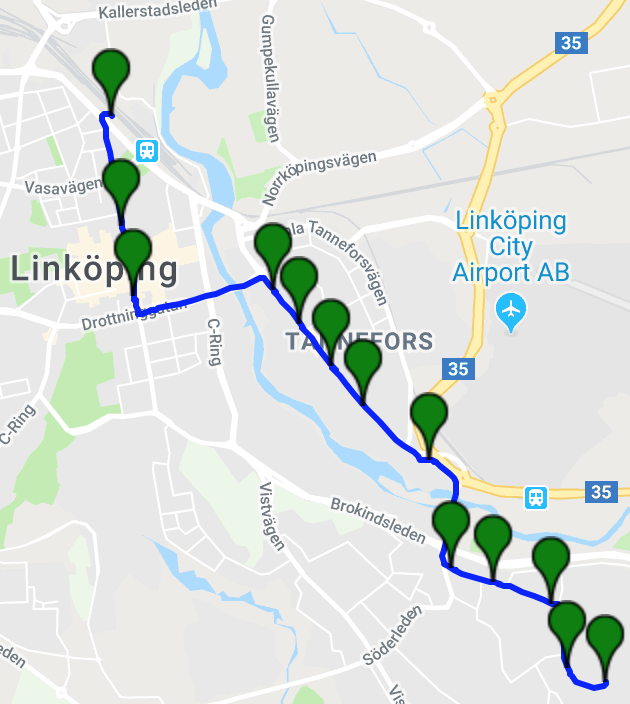
\includegraphics[scale=0.48,width=\textwidth]{211_stations}
	\caption{This figure shows a whole journey of the bus line 211. The markers in green are entered events. Those events have been used to segment the stations.}
	\label{fig:211_stations}
\end{minipage}
\hspace{5pt}
\begin{minipage}{.48\textwidth}
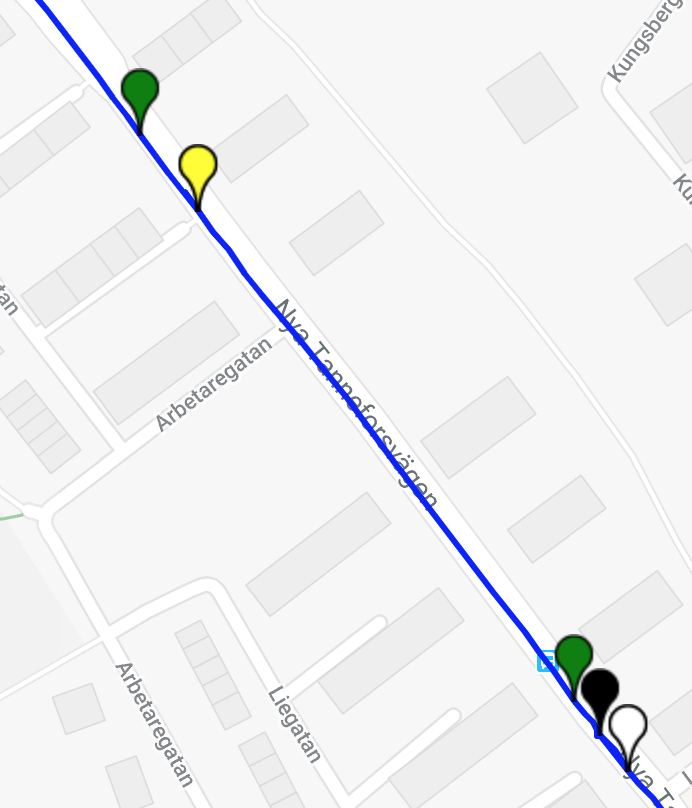
\includegraphics[scale=0.5,width=\textwidth]{entered}
\caption{This caption shows two stations,  the passed the upper left one without stopping, while in the lower right station the bus is stopping.}
\label{fig:entered}
\end{minipage}
\end{figure}


\subsection{Detecting Segments}
Bus journeys are split into several segments. The \textit{EnteredEvent} is used to detect when a bus is approaching a station, and is also used to split the raw data into segments.  We have first tried to use the \textit{StoppedEvent} for segment detection, but as seen in Figure \ref{fig:entered}, that event is not suitable for that use. Occasionaly, some stations are skipped because there are no people trying to get on or off the bus.
The first segment of a journey starts when a \textit{JourneyStartedEvent} triggers. When all the journeys of interest have been collected from the raw data, the collection is investigated in order to find and remove severe anomalies (such as drivers taking a wrong turn). These faulty journeys are discarded since it is not feasible to create a model which takes such complexity into consideration, given the amount of training data available.

\section{Baseline Method}
As a baseline method for segment time prediction the median for each segment over all training data has been used. To be consistent with the way the other two models measures performance, three separate predictions were made for each segments, for each journey. TODO: explain how MAPE is calculated at different intervals of segment progression here? a separate section? don't want us to repeat the same thing 3 times.

\section{Artificial Neural Networks}
A number of different neural network models were implemented and tested. The models were created using \textit{Keras} on top of \textit{Tensorflow}. The created models were both based on suggestions by papers and new ideas because of the richness of features in the Östgötatrafiken dataset. All models will not be mentioned in this report, only the most significant ones. Featured models will be referenced by their notebook name. The implementation follows a three step process which will be described step-wise below. Each step refers to a unique notebook.

\subsection{Step 1 - Additional Pre-processing}
\textit{Notebook: 1. Pre-processing.ipynb}
\newline
Some additional pre-processing was required to train the ANN models. Most importantly the data needs to be labelled with the true labels used to train the models. Datasets aqcuired from the pre-processing described in section \ref{pre-processing} were complemented with the columns

\begin{itemize}
    \item The time it takes to travel the entire current segment (seconds) - Used in Model 1
    \item The time left until next bus stop (seconds) - Used in Models 2,3,4
    \item The time from the start of the journey to the start of the current segment (seconds) - Used in all models
    \item History with the 3 latest GPS coordinates and speed entries.
\end{itemize}

\noindent The first two columns that are added are used as true labels in the respective models. The third one is a feature which captures conditions earlier in the journey. The last column are used to let the network capture traffic conditions.

\subsection{Step 2 - Model Creation}
Each model was implemented separately. Each notebook containing a model takes the data from the previous step and outputs a new data frame with 

\begin{itemize}
    \item segment number
    \item journey number
    \item speed
    \item prediction
    \item label.
\end{itemize}

Where prediction is calculated once per input entry. This was made with the intent of creating easily comparable models.


\subsubsection{Model 1}
\textit{Notebook: 2. Model creation - M1.ipynb}
\newline
\noindent This model was created based on the structure described by Fan and Gurmu \cite{brazilANN}. The model predicts the time it takes to travel the current segment. It is assumed that the time is known when the bus left the latest station. Then, the time left to the next station is calculated by subtracting the time that has passed from the current station from the segment travel time prediction.

\subsubsection{Features}

\begin{itemize}
    \item Segment number (one-hot-encoded)
    \item Time of day (hour), cyclical
    \item Time traveld until the start of the current segment, normalized.
\end{itemize}

%model = keras.Sequential([
%	keras.layers.Dense(2*len(train_data.columns), activation=tf.nn.relu, input_shape=(train_data.shape[1],)),
%    keras.layers.Dense(1*len(train_data.columns), activation=tf.nn.tanh),
%    keras.layers.Dense(1*len(train_data.columns)),
%	keras.layers.Dense(1, activation=tf.nn.relu)
%	])

%optimizer = keras.optimizers.Adadelta()
%model.compile(loss='mae', optimizer = optimizer, metrics=['mae'])

\subsubsection{Layers}

\begin{itemize}
    \item 1 fully connected layer, \textit{2 * \# features} neurons with \textit{RelU} activation function
    \item 2 fully connected layers, \textit{\# features} neurons with activation functions \textit{tanh} and \textit{none} respectively
    \item 1 output neuron with \textit{RelU} activation function
\end{itemize}

This model was obtained using parameter tuning.


\subsubsection{Model 2}\label{M2}
\textit{Notebook: 2. Model creation - M2.ipynb}
\newline
\noindent With this model, the idea was to let the model itself predict the time left to the next segment, in contrast to Model 1. In addition, more features are added.

\subsubsection{Features}

\begin{itemize}
    \item Segment number (one-hot-encoded)
    \item Time of day (hour), cyclical
    \item Time traveld until the start of the current segment, normalized
    \item Bus direction (degrees), cyclical
    \item Bus speed (meter / second), normalized
    \item Bus position (latitude / longitude), normalized
\end{itemize}
  
%    \item Time of day (hour) normalized and (decircled)<- bättre ord tack?
%    \item Time traveld until current segment.
%    \item Direction of the bus
%    \item Speed of the bus
%    \item position of the bus

\subsubsection{Layers}

\begin{itemize}
    \item 1 fully connected layer, \textit{2 * \# features} neurons with \textit{RelU} activation function
    \item 2 fully connected layers, \textit{\# features} neurons with activation functions \textit{tanh} and \textit{none} respectively
    \item 1 output neuron with \textit{RelU} activation function
\end{itemize}

This model was obtained using parameter tuning.

\subsubsection{Model 3}\label{M3}
\textit{Notebook: 2. Model creation - M3.ipynb}
\newline
\noindent This model is very similar to Model 2 with the addition of history from the three latest samples of position and speed data.

\subsubsection{Features}

\begin{itemize}
    \item Segment number (one-hot-encoded)
    \item Time of day (hour), cyclical
    \item Time traveld until the start of the current segment, normalized
    \item Bus direction (degrees), cyclical
    \item Bus speed (meter / second), normalized
    \item Bus position (latitude / longitude), normalized
    \item Bus position history from 3 samples ago (latitude / longitude), normalized
    \item Bus speed history from 3 samples ago (meter / second), normalized
\end{itemize}

\subsubsection{Layers}

\begin{itemize}
    \item 1 fully connected layer, \textit{2 * \# features} neurons with \textit{RelU} activation function
    \item 2 fully connected layers, \textit{\# features} neurons with activation functions \textit{tanh} and \textit{none} respectively
    \item 1 output neuron with \textit{RelU} activation function
\end{itemize}

This model was obtained using parameter tuning.

\subsection{Model 4}
\textit{Notebook: 2. Model creation - M4.ipynb}
\newline
\noindent This model takes a different approach than model 3 to take the history into account. It is a recurrent neural network taking a sequence of 20 consecutive data points as input. It is predicting the time left to the next bus stop like model 2 and 3. 
<Referera RNN pappret?>

\subsubsection{Features}
A sequence of 20 consecutive data points with the following features. 
\begin{itemize}
    \item Segment number (one-hot-encoded)
    \item Time of day (hour), cyclical
    \item Time traveld until the start of the current segment, normalized
    \item Bus direction (degrees), cyclical
    \item Bus speed (meter / second), normalized
    \item Bus position (latitude / longitude), normalized
\end{itemize}

\subsubsection{Layers}

\begin{itemize}
    \item 3 LSTM layers, 128 nodes - \textit{Sigmoid activation}
    \item 1 fully connected layer, 32 nodes - \textit{RelU activation}
    \item 1 output neuron
\end{itemize}

%This model predicts the time it will take to travel to the next bus stop. As input this model use time of day normalized to a value in the range [0,1] and the segment for which the observation has been made. The segment input is one-hot encoded meaning that there is an input for each segment in the journey which all have a value of 0 except for the segment of the observation which has the value 1. The network has one fully connected hidden layer with 13 nodes and an output layer with one node. 
%The network uses the \textit{relu} activation function. This model predicts the time in seconds it will take to travel the whole segment. To get a prediction of the time to the next bus stop you need to subtract the actual known time travelled since the previous bus stop from the output of the neural network.

\subsection{Step 3 - Evaluation}
\textit{Notebook: 3. Evaluation.ipynb}
\newline
As a last step, the models were compared with the \textit{Mean Absolute Error} and are presented one random journey at a time. The loss in the model was also compared with the data without the first segment, as this segment showed to often include a lot of dwell time, heavily impacting the performance. Finally, as some papers has shown good results [ref], a Kalman Filter is applied on top of the predictions.

\section{Gaussian Processes regression for trajectory data}
This section presents how trajectory based GP regression is used to predict the arrival times. The core concept of the model is that each trajectory $X_t$ and corresponding arrival time vector $Y_t$ is considered a realisation of a GP which models the function $Y_t = f^{(t)}(X_t)$. When predicting the arrival time of a new trajectory the model computes which GPs it has previously observed that best explain the new data, and uses the most similar trajectories to make its prediction. However, there are some hurdles with this approach, since trajectories by nature are not synchronised and thus hard to compare in a meaningful way. This is solved by synchronising the trajectories using a separate GP before making the actual predictions. The remainder of this chapter will present in more detail the two steps of synchronisation and prediction.

\subsection{Synchronisation}
As previously mentioned, the trajectories could not be compared spatially. This was because the buses do not drive \textit{precisely} the same route every time, for reasons such as traffic, weather conditions and road work. To be able to train a model based on comparing trajectories, the trajectories first had to be mapped onto a synchronised space $\tau = [0, 1]$, where they could be compared meaningfully. This was done by training a GP modeling a synchronising function $f^{(r,s)}_s(x, y) : \mathcal{R}^2 \mapsto \tau$ for each route $r$ and segment $s$ on a hand picked trajectory. There were two hurdles with this though. Firstly, the data contained a lot of subsegments with buses standing still, which unevenly distributed the data spatially, making the model prioritise getting said subsegments right. Secondly, a GP model does not guarantee that it models a smooth mapping, which was a critical property for this application. To solve the issue of buses standing still, a technique we call \textit{stop compression} was used, and to force the GP to model a smooth mapping \textit{support data} was added. These two issues and techniques used to solve them are described in more detail in the following corresponding subsections.

\subsubsection{Stop Compression}
Since all buses produced approximately one data point every second, a lot of clustered data points is generated while a bus is standing still on a parking lot before a journey or when encountering a red-light. However; the GPs that was used assumed a fixed lenghtscale, which came with the assumption that the data was uniformly distributed.
\begin{figure}[H]
	\caption{Stop compression comparison}
  \begin{subfigure}[b]{0.5\textwidth}
    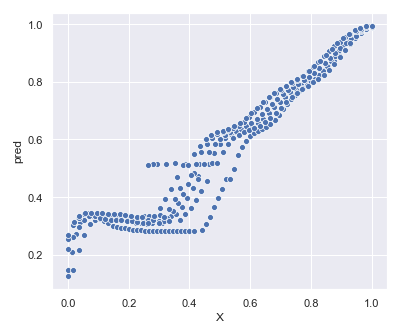
\includegraphics[width=\textwidth]{figures/traj-without-stop-compression.png}
    \caption{Estimated trajectory progression for new data without stop compression.}
    \label{fig:progression-without-stop-compression}
  \end{subfigure}
  %
  \begin{subfigure}[b]{0.5\textwidth}
    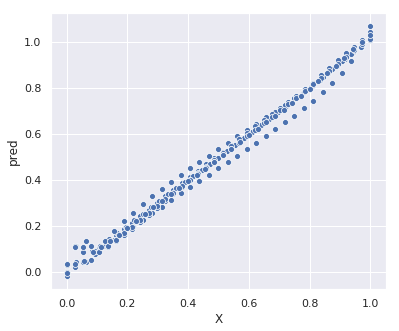
\includegraphics[width=\textwidth]{figures/traj-with-stop-compression.png}
    \caption{Estimated trajectory progression for new data with stop compression.}
    \label{fig:progression-with-stop-compression}
  \end{subfigure}
\end{figure}
\noindent
This assumption did not hold with data points clustered on the same spot, so to make the assumption work, all the data points generated during a stand-still were clustered into one with the mean values of all clustered points. Without this compression, the trajectory used to learn $f^{(r,s)}_s$ also mattered a lot, since where it stopped during a journey would greatly affect the estimated synchronisation function. As shown in figures~\ref{fig:progression-without-stop-compression} and~\ref{fig:progression-without-stop-compression}, the estimated progression much more closely resemble the actual progression when stop compression is used, indicated by the linear relationship.

\subsubsection{Support Data}
In addition to requiring the data to be uniformly distributed, it was essential that $f^{(r,s)}_s$ was a smooth mapping with respect to the direction of spatial progress. That is, data points close in spatial progression should be mapped onto points in $\tau$ which are also close by. Furthermore, data distributed orthogonally to the direction of spatial progression should be mapped onto the same point in $\tau$. This requirement is quite reasonable when one considers that a bus driving slightly more to the left on a road is no closer to its destination than a bus driving slightly more to the right. Another motivation for this is that the GPS data includes some measurement error which has to be considered in the synchronisation.

\begin{figure}[H]
	\caption{Spacial progression}
  \begin{subfigure}[b]{0.5\textwidth}
    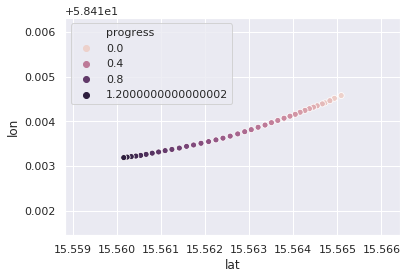
\includegraphics[width=\textwidth]{figures/traj-without-support-data.png}
    \caption{Spatial progression of trajectory 2.}
    \label{fig:traj-without-support-data}
  \end{subfigure}
  %
  \begin{subfigure}[b]{0.5\textwidth}
    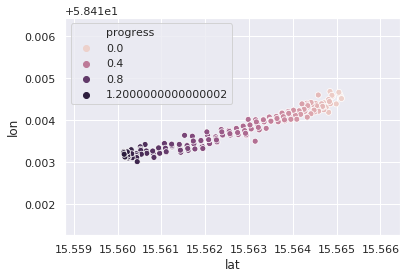
\includegraphics[width=\textwidth]{figures/traj-with-support-data.png}
    \caption{Spatial progression of support data 2.}
    \label{fig:traj-with-support-data}
  \end{subfigure}
\end{figure}
\noindent
In order to force the GP to model a function with this property, each data point $d^{(i)}$ was duplicated by placing a normal distribution over it, orthogonal to the spatial progression vector ${(d^{(i+1)}_x - d^{(i)}_x, d^{(i+1)}_y - d^{(i)}_y)}^T$, and drawing several samples with the same progression as $d^{(i)}$. This process is illustrated in figures~\ref{fig:traj-without-support-data} and~\ref{fig:traj-with-support-data}. The generated support data was saved to a separate data set and combined with the trajectory data when training synhronisation GPs.

\begin{figure}[H]
		\caption{Support data comparison}
  \begin{subfigure}[b]{0.5\textwidth}
    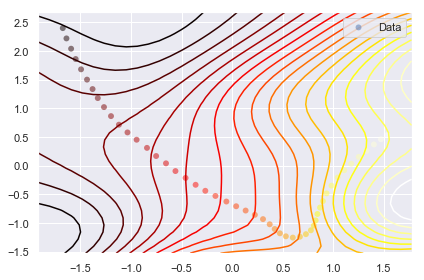
\includegraphics[width=\textwidth]{figures/heat-without-support-data.png}
    \caption{Heightmap of a synchronisation GP without using support data.}
    \label{fig:heightmap-without-support}
  \end{subfigure}
  %
  \begin{subfigure}[b]{0.5\textwidth}
    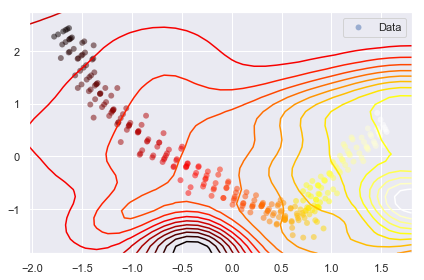
\includegraphics[width=\textwidth]{figures/heat-with-support-data.png}
    \caption{Heightmap of a synchronisation GP using support data.}
    \label{fig:heightmap-with-support}
  \end{subfigure}
\end{figure}
\noindent
As shown in figures~\ref{fig:heightmap-without-support} and~\ref{fig:heightmap-with-support}, using support data greatly increase how orthogonal the contours of $f^{(r,s)}_s$ are to the spatial progression, which indicate the desired properties.

\subsection{Prediction}
After the synchronisation GPs was trained it was possible to train the model for making the actual predictions. Training was done by first mapping all the training trajectories onto $\tau$ using the set of learned  $f^{(r,s)}_s$, and then training two GPs to the synchronised trajectory. The first one was the inverse of the synchronisation GP, ${GP_s^{(t, r,s)}}^{-1}$, which modeled ${f^{(t, r,s)}_s}^{-1}(\tau) : \tau \mapsto \mathcal{R}^2$, and the second was the actual prediction GP $GP_p^{(t,r,s)}$, which modeled ${f^{(t,r,s)}_p}^{-1}(\tau) : \tau \mapsto \mathcal{R}$, which predicted arrival time as a scalar from synchronised progression. Both of these were stored to disk, to be loaded as needed when presented with a new trajectory on the corresponding segment $(r, s)$.

The purpose of ${GP_s^{(t,r,s)}}^{-1}$ was to acquire log likelihoods for new data $(\bar{x}, \bar{y})$, which was given by
\begin{equation}
  \label{eq:model-log-likelihood}
  \begin{split}
    \log P(\bar{y}|\bar{x}, {GP_s^{(t, r,s)}}^{-1}) & = -\frac{1}{2}(\bar{y} - \mu(\bar{x}){[\Sigma]}^{-1}(\bar{x} - \mu(\bar{y}) \\
    & = -\frac{1}{2}\log{|\Sigma|}+C,
  \end{split}
\end{equation}
where $\mu(\bar{x})$ and $\Sigma(\bar{x})$ are given by equations~\ref{eq:gp-mean-function}, and~\ref{eq:gp-variance-function} for a specific ${GP_s^{(t, r,s)}}^{-1}$. Since ${GP_s^{(t,r,s)}}^{-1}$ and $GP_p^{(t,r,s)}$ were trained on the same $t$, it was true that $\log P(\bar{y}|\bar{x}, GP_p^{(t, r,s)})$ was also given by equation~\ref{eq:model-log-likelihood}, which with Bayes theorem gave the unnormalised log distribution
\begin{equation}
  \label{eq:model-log-model-probability}
  \log P(GP_p^{(t, r,s)} | \bar{y}, \bar{x}) \propto \log P(\bar{y}|\bar{x}, GP_p^{(t, r,s)}) + \log P(GP_p^{(t, r,s)})
\end{equation}
over models, where a uniform prior was assumed. The prediction for a model was then given by
\begin{equation}
  \label{eq:model-prediction-probability}
  P(\bar{y}|\bar{x}, GP_p^{(t, r,s)}) \propto P(\bar{y}|\bar{x}, GP_p^{(t, r,s)})P(GP_p^{(t, r,s)} | \bar{y}, \bar{x})
\end{equation}
where Bayes theorem was once again used.
\begin{figure}[H]
	\caption{Density comparison}
  \begin{subfigure}[b]{0.5\textwidth}
    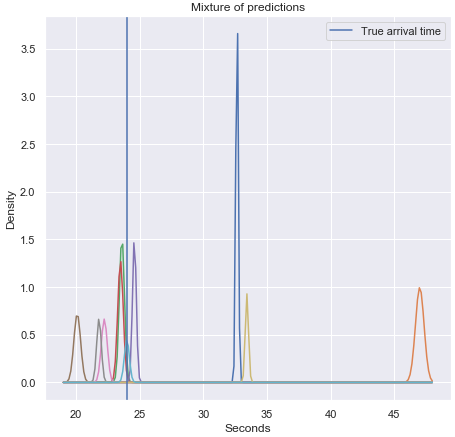
\includegraphics[width=\textwidth]{figures/mixture-start-of-traj.png}
    \caption{Density of arrival times at the start of a segment.}
    \label{fig:mixture-start-of-traj}
  \end{subfigure}
  %
  \begin{subfigure}[b]{0.5\textwidth}
    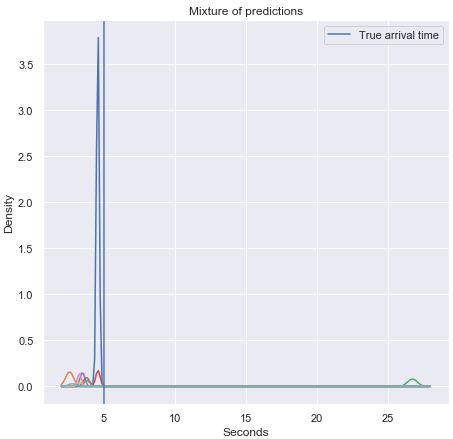
\includegraphics[width=\textwidth]{figures/mixture-end-of-traj.png}
    \caption{Density of arrival times at the end of a segment.}
    \label{fig:mixture-end-of-traj}
  \end{subfigure}
\end{figure}
\noindent
The distribution over arrival times $P(\bar{y} | \bar{x})$ was finally given by a mixture of predictions
\begin{equation}
  \label{eq:model-mixture}
  \sum_{t}{P(\bar{y}|\bar{x}, GP_p^{(t, r,s)})}
\end{equation}
for all trajectories previously trained on. The model made predictions by taking the mean of this distribution. Figure~\ref{fig:mixture-start-of-traj} and figure~\ref{fig:mixture-end-of-traj} show how the models certainty grow as a trajectory progresses, which is because more and more patterns are revealed as more data is collected, which improves the weightings in the mixture distribution.

%%%%%%%%%%%%%%%%%%%%%%%%%%%%%%%%%%%%%%%%%%%%%%%%%%%%%%%%%%%%%%%%%%%%%%
%%% lorem.tex ends here

%%% Local Variables: 
%%% mode: latex
%%% TeX-master: "demothesis"
%%% End: 
